\documentclass{article}
\usepackage{amsmath}
\usepackage[parfill]{parskip}
\usepackage{adjustbox}
\usepackage{listings}
\usepackage{graphicx}
\usepackage{color}
\usepackage{hyperref}
\hypersetup{
    colorlinks,
    citecolor=black,
    filecolor=black,
    linkcolor=black,
    urlcolor=black
}
\graphicspath{ {img/} }
\newcommand{\Mod}[1]{\text{ mod }#1}

\lstset{basicstyle=\ttfamily,
  mathescape=true,
  escapeinside=||}

\begin{document}
\title{COMP8411 - Cryptography and Network Security}
\author{Christopher Williamson}
\maketitle
\tableofcontents
\newpage
\section{Introduction}
Cryptography is `the art of keeping messages secure' by scrambling messages so that they can't be understood by unauthorised people.
\begin{itemize}
	\item Plaintext: a message in its original form
	\item Ciphertext: a message in encrypted form
	\item Encryption: code a message to hide its meaning
	\item Decryption: convert an encrypted message back to its original form
	\item Cryptanalysis: attempts to discover plaintext or key
\end{itemize}

\section{The XOR Operator}
\begin{enumerate}
	\item You can apply XOR in any order: $a \oplus b = b \oplus a$, no matter what values $a$ and $b$ are.
	\item Any bit XOR itself is 0: $a \oplus a = 0$.
	\item Any bit XOR 0 is that bit again e.g. if $a$ is 0 then $0 \oplus 0 = 0$, if $a$ is 1 then $1 \oplus 0 = 1$.
\end{enumerate}
The following rules imply that $a \oplus b \oplus a = b$. We'll use this property when using XOR for encryption. The first XOR with $a$ ($a \oplus b$) is the encryption and the second one is the decryption.

\subsection{One-time pads}
This is an encryption scheme that involves a sequence (the `pad') of random bits that is used as the encryption/decryption key. If the bits are truly random and the pad is only used once, the attacker learns nothing about the plaintext when they see the ciphertext. This property is called \textit{perfect security}.

\subsubsection{Reusing the `one-time' Pad}
Suppose an attacker gets two ciphertexts that have been encrypted with the same key. The attacker can then XOR the two ciphertexts, which is also the XOR of the plaintexts.
\begin{center}
	\begin{tabular}{lcll}
	$c1 \oplus c2$ & $=$ & $(p1 \oplus k) \oplus (p2 \oplus k)$ & (definition) \\
	& $=$ & $p1 \oplus k \oplus p2 \oplus k$ & (reorder terms) \\
	& $=$ & $p1 \oplus p2 \oplus k \oplus k$ & ($a \oplus b = b \oplus a$) \\
	& $=$ & $p1 \oplus p2 \oplus 0$ & ($x \oplus x = 0$) \\
	& $=$ & $p1 \oplus p2$ & ($x \oplus 0 = x$) \\
	\end{tabular}
\end{center}
To extract either $p1$ or $p2$, you'd need to know the other plaintext. The problem is that even the result of the XOR operation on two plaintexts contains quite a bit of information about the plaintexts themselves.

\subsubsection{Remaining Problems}
One-time pads are rarely used due to the fact that the key is at least as large as all of the information you'd like to transmit. You also need to ensure that the keys are exchanged securely ahead of time with all of the people you want to communicate with.

Since the keys have to consist of truly random data for it's security property to hold, key generation is fairly difficult and time-consuming without specialised hardware.

\section{Block Ciphers}
A block cipher is an algorithm that allows us to encrypt blocks of a fixed length. It provides an encryption function $E$ that turns plaintext blocks $P$ into ciphertext blocks $C$, using a secret key $k$:
\begin{center}
	$C = E(k, P)$
\end{center}
Once we've encrypted the plaintext blocks into ciphertext blocks, they later have to be decrypted to recover the plaintext. This is done using a decryption function $D$, which takes the ciphertext block $C$ and the key $k$ and returns the original plaintext block $P$.
\begin{center}
	$P = D(k, C)$
\end{center}
Block ciphers are an example of a symmetric-key encryption scheme, also known as a secret-key encryption scheme. This means that the same secret key is used for both encryption and decryption.

A block cipher is a \textit{keyed permutation}. It's a permutation because it maps every possible block to some other block and it's also a \textit{keyed} permutation because the key determines exactly which blocks map to which. This results in a system where knowing a bunch of (input, output) pairs for a given key shouldn't give you any information about any other pairs under that key.

Below are some design criteria for block ciphers:
\begin{itemize}
	\item Completeness - Each bit of the output should depend on every bit of the input and every bit of the key.
	\item Avalanche effect - Changing one bit in the input should change many bits in the output. Also, changing one key bit should result in the change of many bits in the output.
	\item Statistical independence - Input and output should appear to be statistically independent.
\end{itemize}

\subsection{Feistel Block Cipher}
The operation overview for the Feistel block cipher is as follows:
\begin{enumerate}
	\item Initial permutation of bits
	\item Split in half (left \& right)
	\item 16 rounds of identical operations, but each round uses a different sub key
	\item Inverse initial permutation
\end{enumerate}
\begin{center}
	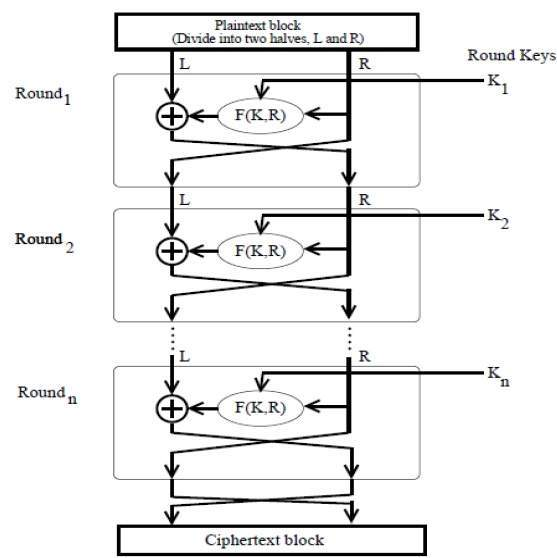
\includegraphics[scale=0.6]{feistel_structure.jpg}
\end{center}
The round function $f$ typically uses permutations, substitutions and modular arithmetic. It take an $n$-bit block and returns an $n$-bit block. A larger block size, $n$, means greater security but makes encryption/decryption slower. It is typically 128 or 256 bits. The key size follows the same principles, 128-bits is the norm. Finally, the number of rounds, $r$ is usually over 10.

\subsection{Data Encryption Standard (DES)}
DES was first published in 1977 as a US Federal standard and is a de facto international standard for banking security. it's a feistel block cipher whose block length is 64 bits and key is 56 bits. The sub-keys, $k1, k2...k16$ are each 48-bits and are generated from the main key. The decryption algorithm is exactly the same as the encryption algorithm except that the keys for each round must be used in reverse order.

\subsubsection{DES Round Function}
\begin{enumerate}
	\item Expansion permutation - Right half is expanded (and permuted) to 48 bits. This diffuses the relationship of input bits to output bits.
	\item Use of round key - All 48 bits of the round key are XOR-ed with out 48 bits from step 1.
	\item Splitting - The result is split into eight lots of six bits each.
	\item S-box (substitution) - Each six bit block is used as an index to an S-box to produce a 4 bit result (so we'll get eight 4 bit blocks).
	\item P-box (permutation) - The 32 bits of output from step 4 are permuted which gives us the output of our round function.
\end{enumerate}
For the S-box step there are 8 different S-boxes, one for each block. Each of these is a table of four rows and 16 columns. The 6 input bits specify which row and column to use for the index of the table. Bits 1 and 6 select the row, bits 2-5 select the column. The decimal value in that cell is then converted to a 4-bit result.

\subsubsection{Triple DES}
Triple DES involves the use of two or three DES keys.

EDE2 is triple DES using two keys, therefore the key length is 112 bits:
\begin{center}
	$C=E_{K1}(D_{K2}(E_{K1}(M)))$
\end{center}
EDE3 is triple DES using three keys, therefore the key length is 168 bits:
\begin{center}
	$C=E_{K3}(D_{K2}(E_{K1}(M)))$
\end{center}

\subsection{Advanced Encryption Standard (AES)}
This is the most common block cipher in current use. It was selected through a public, peer-reviewed competition.
\begin{itemize}
	\item Block size: 128 bits (called a state)
	\item Key sizes: 128, 192 or 256 bits
\end{itemize}
AES consists of several independent steps. At a high level, AES is a substitution-permutation network involving $r$ rounds.
\begin{center}
	\begin{tabular}{|c|c|}
		\hline
		Key length & Rounds \\ \hline
		128 & 10 \\
		192 & 12 \\
		256 & 14 \\
		\hline
	\end{tabular}
\end{center}
A single round transformation consists of the following steps:
\begin{itemize}
	\item Byte substitution.
	\item Shift rows.
	\item Mix columns.
	\item Round key addition.
\end{itemize}
Note that in practice, the round key addition step if done before the rounds start, and in the last round, the mix columns step is not performed.

\subsubsection{Byte Substitution}
The SubBytes transformation is a simple table lookup. There is only one S-box (substitution box) for the while cipher, a 16x16 matrix of byte values that contains a permutation of all possible 256 8-bit values. Each individual byte of \textbf{state} is mapped into a new byte in the following way:
\begin{itemize}
	\item Leftmost 4 bits of the byte are used as a row value; rightmost 4-bits are used as a column value.
	\item These row and column values serve as indexed into the S-box to select a unique 8-bit output value
\end{itemize}

\subsubsection{Shift Rows}
For this step we first put the bytes into a 4x4 grid. The first 4 bytes on the top row, 5-8 on the second etc. The following permutations then occur:
\begin{itemize}
	\item 1st row: not altered
	\item 2nd row: a 1-byte circular left shift
	\item 3rd row: a 2-byte circular left shift
	\item 4th row: a 3-byte circular left shift
\end{itemize}
The decryption process uses shifts to the right. This step permutes bytes between the columns.

\subsubsection{Mix Columns}
Mix columns multiplies each column of the state with a fixed polynomial. Shift rows and mix columns represent the diffusion properties of AES.

\subsubsection{Add Round Key}
In this step, each byte of the state is combined with the round key using XOR i.e. the 128 bits of state are bit-wise XORed with the 128 bits of the round key.

\subsubsection{Pseudocode (AES-128)}
\begin{lstlisting}
addRoundKey(S, K[0]);

for (i = 1; i <=9; i++) {
    subBytes(S);
    shiftRows(S);
    mixColumns(S);
    addRoundKey(S, K[i]);
}

subBytes(S);
shiftRows(S);
addRoundKey(S, K[10]);
\end{lstlisting}

\subsection{DES vs AES}
\begin{center}
	\begin{tabular}{p{6cm}p{6cm}}
		\multicolumn{1}{c}{\textbf{DES}} & \multicolumn{1}{c}{\textbf{\textbf{AES}}} \\
		Substitution-permutation, iterated cipher, feistel structure & Substitution-permutation, iterated cipher \\
		64-bit block size, 56-bit key size & 128-bit block size, 128-bit (192, 256) key sizes \\
		8 different S-boxes & 1 S-box \\
		Design optimised for hardware implementations & design optimised for byte-orientated implementations. \\
		Closed (secret) design process & Open design and evaluation process \\
	\end{tabular}
\end{center}

\subsection{Other Symmetrical Cryptosystems}
\begin{center}
	\begin{tabular}{|l|l|l|}
	\hline
	Algorithms & Mode (block length in bits) & Key length (bits) \\ \hline
	DES & Block cipher (64) & 56 \\ \hline
	Triple DES & Block cipher (64) & 168 $(=3*56)$ (112 effective) \\ \hline
	Rijndael & Block cipher (128, 192 or 256) & 128, 192 or 256 \\ \hline
	Blowfish & Block cipher (64) & variable up to 448 \\ \hline
	IDEA & Block cipher (64) & 128 \\ \hline
	RC5 & Block cipher (32, 64, 128) & Variable up to 2040 \\
	\hline
	\end{tabular}
\end{center}

\subsection{Modes of Operation - Encrypting Large Messages}
If a message is longer than its block size, the block cipher can be used in a variety of ways to encrypt the plaintext. There are a number of modes of operations, below are three of them:
\begin{itemize}
	\item ECB - Electronic Code Book mode
	\item CBC - Cipher Block Chaining mode
	\item CTR - Counter mode
\end{itemize}
These modes of operation have been standardised internationally and are applicable to any block ciphers.

\subsubsection{ECB Mode}
In this mode, each block is encrypted independently using the same key. The last block should be padded if necessary. Usually the last byte indicates the number of padding bytes added; this allows the receiver to remove the padding. The blocks are then encrypted independently of each other. Reordering the ciphertext blocks will result in correspondingly reordered plaintext blocks.

\subsubsection{CBC Mode}
In this mode the plaintext is divided into blocks and the last block is padded if necessary. Ciphertext block $C_{j}$ depends on plaintext block $M_{j}$ \textbf{and all preceding plaintext blocks}:
\begin{center}
	$C_{n} = E_{k}(M_{n} \oplus C_{n-1})$ \\
	$C_{0} = IV$ (Initialisation vector)
\end{center}

\subsubsection{CTR Mode}
A counter, equal to the plaintext block size is used. The counter value must be different for each plaintext block. Typically the counter is initialised to some value, and then incremented by 1 for each subsequent block (modulo $2^{n}$, where $n$ is the block length).

Each block can be decrypted independently of the other, therefore it can be run in parallel and there is also no error propagation.

\subsection{Block Ciphers vs Stream Ciphers}
While block ciphers encrypt blocks of characters, stream ciphers encrypt individual characters or bit streams.

Stream ciphers:
\begin{itemize}
	\item Are usually faster than block ciphers in hardware; mostly used for continuous communications and/or real-time applications.
	\item Requires less memory space, so cheaper for resource restrained devices such as embedded sensors.
	\item Have limited or no error propagation, so advantageous when transmission errors are probable.
	\item Can be build out of block ciphers, e.g. by using CTR modes.
\end{itemize}

\section{Public Key Cryptography}
Up to this point, all cryptographic schemes are based on shared secret-keys (symmetric cryptography). One major problem with symmetric cryptography is that a separate key is needed for each pair of users. Therefore, an $n$-user system requires $n*(n-1)/2$ keys - the $n^{2}$ problem. Generating and distributing these keys is also a challenging problem and maintaining security for already distributed keys is challenging. Finally, as two parties share the same key, non repudiation can not be achieved. It was in 1976 that Diffie and Hellman first presented the concept of public key cryptography.
\begin{itemize}
	\item Based on mathematically hard problems rather than substitution/transposition.
	\item A pair of keys is used, public and private. Pair are related mathematically.
	\item Encryption generated by one key can only be decrypted by the other key in that pair.
	\item Examples: RSA, DSS, DH (Diffie Hellman).
\end{itemize}

\subsection{Achieving Confidentiality}
Our scenario is that Alice wants to send a message to Bob and ensure that is has confidentiality protection.
\begin{enumerate}
	\item Alice encrypts the message with Bob's \textbf{public} key
	\item Bob decrypts Alice's message with his \textbf{private} key
\end{enumerate}
This method ensures that only Bob can decrypt the ciphertext (as he is the only one in possession of his private key). Usually this is only applied to short messages, e.g. for secure transmission of symmetrical keys.

\subsection{Achieving Authenticity}
Our scenario here is that Alice wants to send a message to Bob and Bob wants to be assured that the message has come from Alice.
\begin{enumerate}
	\item Alice signs the hash value of the plaintext with her \textbf{private} key
	\item Bob verifies the hash value using Alice's \textbf{public} key
\end{enumerate}
Usually the signature is signed in the hash value of the plaintext, and a timestamp should also be included.

\subsection{Modulo Operator}
\begin{center}
	$a \equiv b \Mod n$
\end{center}
Means that there exists an integer number $k$ such that $a$ can be represented as:
\begin{center}
	$a \equiv k \cdot n + b$
\end{center}
Given integers, $a$, $b$, and $n \neq 0$. $a$ is congruent to $b \Mod n$ iff $a-b \equiv k\cdot n$ for some integer $k$.

Examples:
\begin{itemize}
	\item $9 \Mod 5 = 4$
	\item $20 \Mod 9 = 2$
	\item $17 = 2 \Mod 5$ since $17-2 = 3 \cdot 5$
\end{itemize}
Below are some properties of modular arithmetic:
\begin{itemize}
	\item $a \equiv a \Mod n$
	\item $a \equiv b \Mod n \leftrightarrow b \equiv a \Mod n$
	\item $a \equiv b \Mod n \text{ \& } b \equiv c \Mod n \rightarrow a \equiv c \Mod n$
	\item $(a + b) \Mod n = ((a \Mod n) + (b \Mod n)) \Mod n$
	\item $(a \cdot b) \Mod n = ((a \Mod n) \cdot (b \Mod n)) \Mod n$
	\item $a \cdot (b + c) \Mod n = (a \cdot b + a \cdot c) \Mod n$
	\item $a \cdot x \Mod n = 1$ where $x$ is an integer and called the multiplicative inverse of $a$
\end{itemize}
Below is some code that finds the multiplicative inverse of $a$ under $n$:
\begin{lstlisting}
def multiplicative_inverse(a, n):
  x = 1

  while x < n:
    if (a*x) % n == 1:
      return x
    else:
      x += 1
\end{lstlisting}
$a$ and $b$ are said to be relatively prime if only 1 can divide each of them e.g. 8 and 15.
\subsection{RSA Algorithm}
The RSA algorithm was invented by Ron \textbf{R}ivest, Ali \textbf{S}hamir and Leonard \textbf{A}dleman. It has withstood years of cryptanalysis and remains by far the most popular and well trusted scheme.

The algorithm consists of two numbers, the modulus, $n$, and the public exponent, $e$. The modulus is a product of two very large prime numbers (100 to 400 digits), represented by the letters $p$ and $q$. They need to be kept secret.

It is a block cipher in which the plaintext and ciphertext are integers between 0 and $n-1$ for some $n$.

\subsubsection{Key Generation}
\begin{enumerate}
	\item Select two large primes, $p$ and $q$
	\item Calculate $n = p \cdot q$ and $\phi(n) = (p-1) \cdot (q-1)$
	\item Select an integer, $e$ which is relatively prime to $\phi(n)$ and $1 < e < \phi(n)$
	\item Calculate a value $d$ such that $d = e^{-1} \Mod \phi(n)$ or $(d \cdot e) \Mod \phi(n) = 1$
	\item Public key = ${e, n}$
	\item Private key = ${d, n}$
\end{enumerate}
You can see that $e$ is \textbf{publicly} chosen and $d$ is \textbf{private} and calculated.

\subsubsection{Encryption}
For the plaintext, we represent it as an integer $M$ in the range $0 < M < n$. The ciphertext is then:
\begin{center}
	$C = M^{e} \Mod n$
\end{center}

\subsubsection{Decryption}
To get the plaintext from the ciphertext we use the private key, ${d, n}$:
\begin{center}
	$M = C^{d} \Mod n$
\end{center}

\subsubsection{Worked Example}
\begin{enumerate}
	\item Select $p=7$ and $q=17$
	\item Calculate $n = p \cdot q = 119$
	\item Calculate $\phi(n) = (p-1) \cdot (q-1) = 96$
	\item Select $e = 5$, which is relatively prime and less than $\phi(n)$
	\item Calculate $d=77$ such that $de \Mod \phi(n) = 1$
	\item Let $M = 19$, then $C = 19^{5} \Mod 119 = 66$
\end{enumerate}

PKCS\#1 standard defines the use of the RSA algorithm. It defines the key generation, encryption, decryption, digital signatures, verification, public key format, padding, and several other issues with RSA: \url{https://en.wikipedia.org/wiki/PKCS_1}

The security of RSA relies on the difficulty of finding $d$ given ${e, n}$. $p$ and $q$ should differ in length by only a few digits, and both should be on the order of 100 - 200 digits or even larger.
\begin{itemize}
	\item $n$ with 150 digits could be factored in about 1 year
	\item Factoring $n$ with 200 digits could take about 1000 years
\end{itemize}
\subsection{Hybrid Cryptosystems}
Public key ciphers are much slower than symmetrical key ciphers, 1000 times slower in hardware, and 100 times slower in software, than DES. Symmetric ciphers also have key management problems and can not provide non-repudiation service without the involvement of a trusted third party.

Due to these issues, we usually combine them to get the strengths of both - this leads to the hybrid cryptosystem:
\begin{itemize}
	\item Public cipher for symmetric key establishment/transportation and/or digital signature generation.
	\item Symmetric cipher for bulk encryption.
\end{itemize}
The technique is called digital enveloping. A symmetrical algorithm with a random session key is used to encrypt the message and then a public-key algorithm is used to encrypt the random session key.

\section{Cryptographic Checksums}
Conventional symmetric encryption: $a \rightarrow B: E_{k}[M]$ provides confidentiality, as ONLY $A$ and $B$ share $K$. It also provides a certain degree of origin authentication as it could only come from $A$. It does not provide signature as receiver $B$ could also generate the encryption and sender $A$ could deny sending the message (repudiation of origin).

Public key encryption: $A \rightarrow B: E_{KUb}[M]$ provides confidentiality but not origin authentication as everyone knows $B$s private key.

Digital signing is applied in the following manner:
\begin{center}
  $A \rightarrow B: M \| E_{KR_{a}}[h(M)]$
\end{center}
Which means that we have the plaintext, $M$, with the encrypted hash value of $M$ attached to the end of it. The encryption is done with $A$s private key. This method provides origin authentication and non-repudiation as:
\begin{itemize}
  \item Only $A$ has $KR_{a}$, so signed item must have come from $A$.
  \item Any party can use $KU_{a}$ to verify the item.
  \item Provided $KU_{a}$ is trust-worthy, and the signature is dated.
\end{itemize}
But it does not provide confidentiality.

Some of the cryptographic operations mentioned above could only provide message authentication and integrity protections provided that the message has some structures or is recognisable. We therefore need some redundancy for the receiver to verify the message - this check-value is a \textbf{cryptographic checksum}.

A cryptographic checksum can be used to protect:
\begin{itemize}
  \item Content authentication (origin + integrity)
  \item Non-repudiation
  \item Anti-replay
\end{itemize}

\subsection{Digest Function}
Given a message, $M$, of arbitrary length, a Message Digest function, $H$, produces a fixed-size output, $h$ (called a message digest, checksum, hash value, or fingerprint, of $M$). $h$ should be a function of all the bits of $M$

\subsubsection{Requirements}
A message digest function should take into account the following properties:
\begin{itemize}
  \item \textbf{Compression}: $H$ can be applied to a block of data of any size, but produces a fixed-length output.
  \item \textbf{One-way property}: $H(x)$ is easy to compute for any given $x$. For any given $h$, it is hard to compute $x$ such that $H(x) = h$.
  \item \textbf{Weak collision resistance}: Given $x$, it is hard to find $y \neq x$ such that $H(y) = H(x)$.
  \item \textbf{Strong collision resistance}: It is hard to find two different messages, $x \neq y$, such that $H(y) = H(x)$.
\end{itemize}
If $H$ is strong collision resistant, it is also weak collision resistant.

If the weak collision resistance property is not met signature forgery is likely. Assuming that $A$ has sent a signed message $M$ to $B$, $M \| s$ where $s=R_{KR_{a}}[H(M)]$:
\begin{enumerate}
  \item An attacker intercepts $A$'s signature and message.
  \item The attacker finds another message, $M'$ where $H(M) = H(M')$.
  \item The attacker now has your signature $s$ on the real message.
\end{enumerate}
Repudiation is likely if the strong collision resistance property is not met. Assuming that $A$ is to send a signed message $M$ to $B$:
\begin{enumerate}
  \item $A$ chooses two messages $M$ and $M'$ where $H(M) = H(M')$.
  \item $A$ signs $M$ by generating the signature.
  \item $A$ sends $B$ $M \| s$.
  \item Later $A$ repudiates this signature, saying that it was really a signature on the message $M'$.
\end{enumerate}

\subsection{Construction Methods}
Cryptographic checksum construction methods include message authentication code (MAC), hash functions and HMAC, among others. Below we take a deeper look into some of these construction methods.

\subsubsection{Extension Method}
In this method, each MD function processes a block of $M$, the output is the input for the next block. The output of the final block is the digest of the entire message.

\subsubsection{Message Authentication Code (MAC)}
This is a public function with a shared secret key that produces a fixed-length output i.e. $\text{MAC} = f_{k}(M)$.

It is block cipher based which means that it is slow and produces a short digest length. As before, the output of one block is the input to the next block. At the end we just take the last output value as our digest.

If only $A$ and $B$ know the secret key $K$, and if $\text{MAC} = \text{MAC}'$ (MAC' is the receivers digest), then the receiver can be assured that:
\begin{itemize}
  \item The message has not been altered.
  \item The message is from the alleged sender.
  \item The message is of the proper sequence if the message includes a sequence number.
  \item The message is fresh, if the message includes a timestamp.
\end{itemize}

\subsubsection{Hash Functions}
Below is a table of commonly used hash functions:
\begin{center}
  \begin{tabular}{|l|l|l|l|l|}
    \hline
    & SHA-1 & SHA-256 & SHA-384 & SHA-512 \\ \hline
    Hash value size & 160 & 256 & 384 & 512 \\ \hline
    Block size & 512 & 512 & 1024 & 1024 \\ \hline
    Word size & 32 & 32 & 64 & 64 \\ \hline
    Security & 80 & 128 & 192 & 256 \\
    \hline
  \end{tabular}
\end{center}
Security refers to the fact that a birthday attack on a message digest of size $n$ produces a collision with a work-factor of approximately $2^{n/2}$.

\subsubsection{HMAC}
HMAC constructs MAC by applying a message and key to a cryptographic hash function in a nested manner i.e.
\begin{center}
  $\text{HMAC}(K, M) = H[(K \oplus \text{opad}) \| H[(K \oplus \text{ipad}) \| M)]]$
\end{center}
Where:
\begin{itemize}
  \item \textbf{H}: hash function such as SHA-1
  \item \textbf{ipad}: a string by repeating the byte 0x36 (00110110) as often as necessary.
  \item \textbf{opad}: a string by repeating the byte 0x5c (01011100) as often as necessary.
  \item \textbf{K}: 512-bits secret key
\end{itemize}

\section{Digital Signature Algorithms}
A digital signature associates a mark unique to an individual with a body of text. It should be:
\begin{itemize}
  \item Message-dependent: unreusable \& ensures integrity
  \item Signer-dependent: unforgable \& ensures authenticity
  \item Verifiable: others should be able to verofy that the signature is indeed from the originator.
\end{itemize}
A digital signature scheme uses public-key cryptography, typically RSA or DSA.

The main idea is that only $A$ can sign a message because only $A$ has access to their private key. Anyone can verify $A$'s signature because everyone has $A$'s public key. A digital signature scheme consists of a key generation algorithm, a signature generation algorithm and a signature verification algorithm.

\subsection{RSA for Digital Signature - Problems}
One problem with using RSA for digital signature is that RSA can only handle so much data and we may want to sign a message which is longer than RSA allows. One way to solve this would be to break the message up into smaller chunks but this would add a great deal of complexity and expense.

There is also a security issue:
\begin{itemize}
  \item Let $m$ be the message of which you want to forge a signature.
  \item Choose two messages $x$ and $y$ such that $xy = m \Mod n$.
  \item If you could obtain the signatures of $x$ and $y$ then you can easily forge a signature of $m$ by $S(m) = S(y)S(x) \Mod n$
\end{itemize}
A solution to these problems is to use the `hash-and-sign' paradigm where we sign the hash value of the message. Below is how we write the signature generation process and the signature verification process:
\begin{center}
  $S=E_{KR_{a}}[H(M)]$ \\
  $h=D_{KU_{a}}[S] = D_{KU_{a}}[E_{KU_{a}}[H(M)]]$
\end{center}
The remaining problem is how can we ensure that public keys are trustworthy? This is covered in the Public Key Infrastructure topic.

\subsection{DSA}
Below is an illustration of the workings of the DSA algorithm:
\begin{center}
  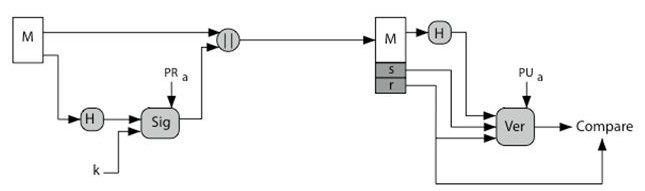
\includegraphics[scale=0.6]{dsa.jpg}
\end{center}
$k$ is a random number generated for this signature (it should be different for every signature generation). $PR_{a}$ is the sender's private key and $PR_{a}$ is the sender's public key.

\subsubsection{Key Generation}
First we generate our global public-key components that can be shared among a group of users:
\begin{itemize}
  \item Choose $p$, a 512-bit to 2048-bit prime number.
  \item Choose $q$, a 160-bit prime number which divides $(p-1)$ ($q$ is a prime divisor of $p-1$).
  \item $g = h^{(p-1)/q} \Mod p$ where $h$ is any integer where $1 < h < (p-1)$ such that $h^{(p-1)/q} \Mod p > 1$.
\end{itemize}
Next, we choose a long-term private key, $x$, which should be a randomly chosen value in the range $0 < x < q$. Now we can compute our long-term public key:
\begin{center}
  $y = g^{x} \Mod p$ \\
  $KU_{a} = \{p, q, g, y\}$
\end{center}

\subsubsection{The Signing Process}
Once we have our public/private key pair, we can move onto the signing stage. First, we choose a random number for $k$. This key must be destroyed after use and must never be reused. We then compute two components:
\begin{itemize}
  \item $r = (g^{k} \Mod p) \Mod q$
  \item $s = [k^{-1}(H(M) + xr)] \Mod q$
  \item $\text{Signature} = (r, s)$
\end{itemize}
We can then send $M \| \text{signature}$ to the receiver.

\subsubsection{Signature Verification}
So now the receiver has got $KU_{a}$ and $\{M', r', s'\}$. We compute:
\begin{itemize}
  \item Message hash $H(M')$
  \item mod $q$ inverse of $s'$: $w = (s')^{-1} \Mod q$
  \item $u_{1} = [H(M')w] \Mod q$
  \item $u_{2} = (r')w \Mod q$
  \item $v = [(g^{u_{1}}y^{u_{2}}) \Mod p] \Mod q$
\end{itemize}
We then test that $v = r'$. If this is true, then the signature is verified.

\subsection{RSA vs DSA}
\begin{tabular}{|p{6cm}|p{6cm}|}
  \hline
  \multicolumn{1}{|c|}{\textbf{RSA}} & \multicolumn{1}{|c|}{\textbf{\textbf{DSA}}} \\ \hline
  Security is based on difficulty of factoring large numbers & Security is based on difficulty of taking discrete logarithms \\ \hline
  Can encrypt and sign & Can only sign messages \\ \hline
  Faster than DSA in signature verification, and about the same in signature generation. & Some signature computation can be computed priori. \\ \hline
  Can recover the message digest from the signature & Cannot recover the message digest from the signature \\ \hline
  & Need to choose a unique secret number $k$ for each message \\
  \hline
\end{tabular}



\end{document}
